\documentclass[t, notes, xcolor=table]{beamer}

\usepackage{wrapfig}
\usepackage{float}
% For tabs in verbatim
\usepackage{fancyvrb}

% Adjust position of the image
\usepackage[export]{adjustbox}

% set fonts
\usefonttheme{professionalfonts} % using non standard fonts for beamer
\usepackage{txfonts,mathptmx}

% set indend spacing for first and second level indentation
\setlength{\leftmargini}{0.5cm}
\setlength{\leftmarginii}{0.5cm}
\setlength{\leftmarginiii}{0.5cm}

% Set circles for bullets 
\setbeamertemplate{itemize items}[circle]

% colors
\usepackage{xcolor}

% multiple columns
\usepackage{multicol}

% todo lists
\usepackage{pifont}
\usepackage{amssymb}

% increase space between text and frame name
\addtobeamertemplate{frametitle}{}{\vspace{0.5em}}

%Information to be included in the title page:
\title{Managing the Logic Synthesis Process}
\author{Nikola Petrovic}
\institute{University of Belgrade, School of Electrical Engineering}
\date{2022}



\begin{document}

\frame{\titlepage}

%%%%%%%%%%%%%%%%%%%%%%%%%%%%%%%%%%%%%%%%%%%%%%%%%%%%%%%%%%%%
\begin{frame}
\frametitle{Module Objective}
\normalsize{
In this module we will go through the Synthesis Flow and manage the Synthesis Process.
\newline

\textbf{Topics:}
\begin{itemize}
\item Reading the HDL source
\item Elaborating the design
\item Applying constraints
\item Mapping to technology cells
\item Writing the netlist
\item Optimizing Arithmetic Expressions
\item Sharing/un-sharing Resources
\item Boundary optimization, Re-timing, Scan Insertion
\item Analyzing Results, Report Timing
\end{itemize}
}
\end{frame}
\note{
\scriptsize{
This module just briefly presents the basic steps of the synthesis process and the associated Cadence Encounter RTL Compiler commands.
\newline

This module expands upon the synthesis process that the first module examined. The flow described here is similar to all popular synthesis tools. Any more exact examples derive from the Cadence Encounter RTL Compiler (RC).

}
}



%%%%%%%%%%%%%%%%%%%%%%%%%%%%%%%%%%%%%%%%%%%%%%%%%%%%%%%%%%%%
\begin{frame}
\frametitle{Logic Synthesis Goals}
\footnotesize{
Work fast

\begin{itemize}
\item Faster than the other guy’s synthesis, definitely faster than manual
\end{itemize}

Work accurately

\begin{itemize}
\item Gate-level model functionally equivalent to RTL model
\item Cost estimates correspond well with actual values measured later
\begin{itemize}
\footnotesize{
	\item[$-$] Area, time, power
}
\end{itemize}
\end{itemize}

Maximize Quality of Silicon (QoS)

\begin{itemize}
\item Minimize time - maximize frequency and throughput
\item Minimize area - cell count and cell size
\item Minimize power - switching activity and leakage power
\end{itemize}
}
\end{frame}
\note{
\tiny{
Synthesis tools, like all tools really, have only the two goals to work fast and work well. This slide further splits from the "work well" part the issue of accuracy, for if the tool does not evaluate function and timing well, who cares how wonderful are the false numbers?
\begin{itemize}
\item Working fast in a modern highly-competitive industry environment means not just optimizing the design faster than I could do it with pencil and paper but also faster than whatever tool my competitor uses. Here, "faster" means not just tool speed, but also tool usability and tool support that come to play.
\item Working accurately, is at least for a modern tool, no longer an issue. Functional accuracy has not been
an issue for decades and is now so rare that it is the highest level bug when encountered. Timing accuracy has for long been mainly an issue of how closely the chosen wire-load tables model actual parasitics of the routed design. Modern synthesis tools work in conjunction with layout tools to greatly
improve timing accuracy.
\item Producing high-quality silicon means minimizing the "cost" factors. Cost factors are foremost timing and only slightly secondarily area and power. All of these cost factors are really just different ways to provide more utility to the customer, i.e., to make the customer want to buy my product instead of the
other guy's:
\begin{itemize}
\tiny{
	\item Timing is important because higher clock speed means that I can put more functionality into a smaller space and have it respond more quickly to my customer's inputs.
	\item Area is important because less area means that I can put more functionality into a smaller space and I can also reduce the price because my own manufacturing and packaging costs are lower.
	\item Power is important because less power dissipation means that my customer has lower energy costs, if it is a portable device then the battery can be lighter and stay charged longer, and if it is a handheld device then the customer does not cook their hand while holding it.
}
\end{itemize}
\end{itemize}

}
}

%%%%%%%%%%%%%%%%%%%%%%%%%%%%%%%%%%%%%%%%%%%%%%%%%%%%%%%%%%%%
\begin{frame}
\frametitle{Logic Synthesis Basic Process}
\begin{multicols}{2}
From RTL input:
\begin{itemize}
\item Parse
\item Translate
\item Optimize
\item Map
\item Optimize again
\item Insert scan
\item Optimize again
\end{itemize}
\vfill
\columnbreak
\begin{figure}
    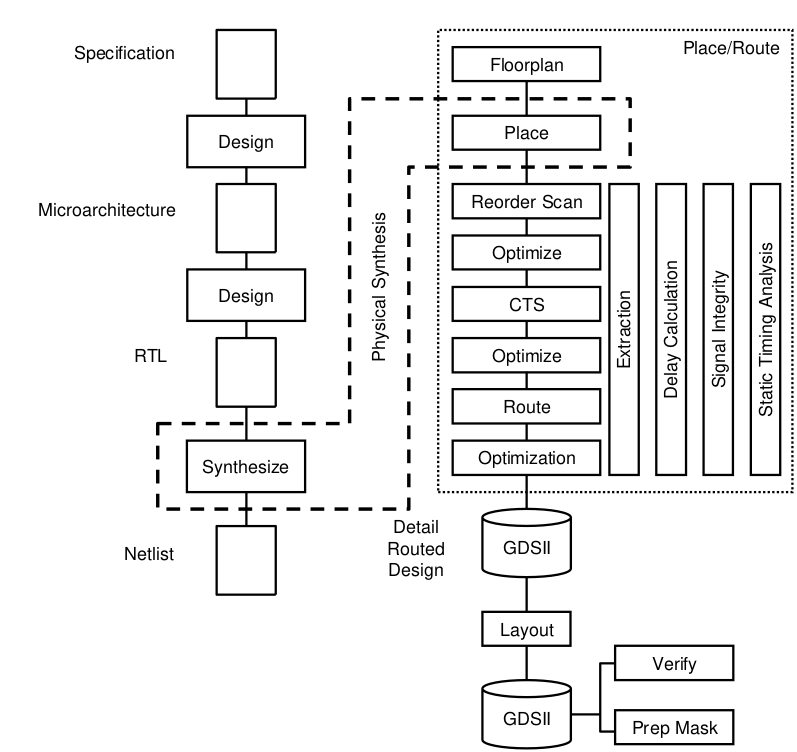
\includegraphics[width=0.5\textwidth,left]{img/17_synth_process.png}
\end{figure}
\end{multicols}
\end{frame}
\note{
\scriptsize{
This module expands somewhat upon the synthesis process that the first module examined, for if you understand something about what's going on inside the flow, then you are likely to provide better-quality RTL inputs.
\newline

After every major operation the tool again optimizes the design. Optimization means calculating the design timing, area and power, and if not within your targets, swapping gates and restructuring logic in an attempt to meet your targets.

}
}

%%%%%%%%%%%%%%%%%%%%%%%%%%%%%%%%%%%%%%%%%%%%%%%%%%%%%%%%%%%%
\begin{frame}
\frametitle{Logic Synthesis Inputs and Outputs}
\begin{multicols}{2}
\textbf{Input}
\begin{itemize}
\item Synthesizable HDL
\item Constraints – (SDC)
\item Technology libraries
\end{itemize}
\vfill
\columnbreak

\textbf{Output}

\begin{itemize}
\item Netlist - (usually Verilog)

\begin{itemize}
	\item Of technology macros
\end{itemize}

\end{itemize}

\end{multicols}
\begin{figure}
    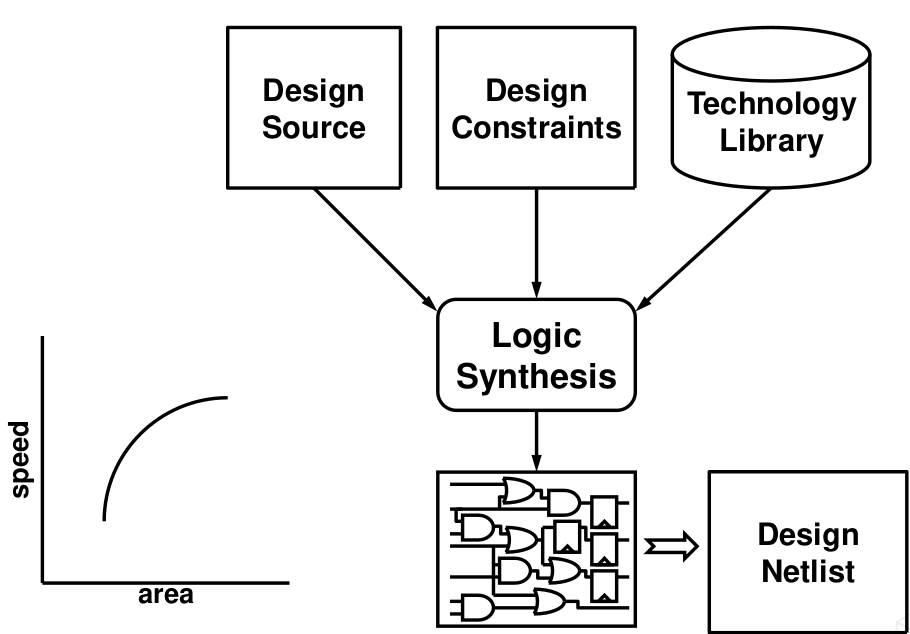
\includegraphics[width=0.65\textwidth]{img/17_synth_inouts.png}
\end{figure}
\end{frame}
\note{
\scriptsize{
Inputs to the synthesis process include:
\begin{itemize}
\item The design itself, written in the "synthesizable subset" of the HDL.
\item Design constraints, including the required clock speed, input drive strength and arrival time with respect to the clock, and output load and required arrival time with respect to the clock. Design constraints can also include power consumption and can sometimes include noise immunity, testability, and factors affecting ease of place and route. Design constraints may be in the Synopsys Design Constraint (SDC) format, and synthesis vendors also have their own proprietary formats.
\item At least one technology library, including all pertinent information about the available cells, and factors for estimating interconnect delays.
\end{itemize}

Outputs from the synthesis process include:
\begin{itemize}
\item Most importantly, the design as a structural netlist of technology cells.
\item Optionally, post-synthesis timing information for annotation to a gate-level simulation.
\item A log file and any other reports you requested from the tool.
\end{itemize}

}
}

%%%%%%%%%%%%%%%%%%%%%%%%%%%%%%%%%%%%%%%%%%%%%%%%%%%%%%%%%%%%
\begin{frame}
\frametitle{Logic Synthesis Basic Flow}
\begin{figure}
    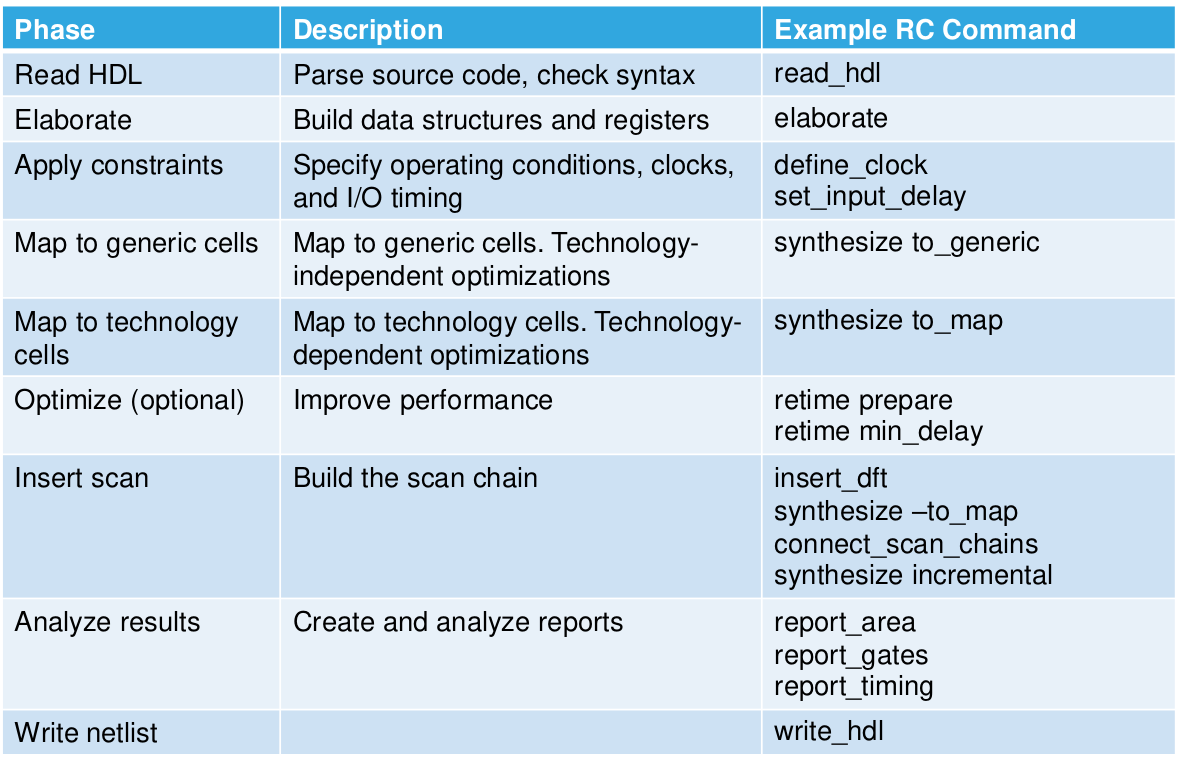
\includegraphics[width=0.95\textwidth]{img/17_synth_flow.png}
\end{figure}
\end{frame}
\note{
\scriptsize{
The remainder of this module examines a generic flow from reading the HDL to writing the optimized netlist. Example commands are those of the Cadence Encounter RTL Compiler. Most of these commands have several options that this training does not show. This training also does not show the complete command set. For example, applying constraints is quite a bit more involved then simply defining the clocks.

}
}

%%%%%%%%%%%%%%%%%%%%%%%%%%%%%%%%%%%%%%%%%%%%%%%%%%%%%%%%%%%%
\begin{frame}[fragile]
\frametitle{Reading HDL}
\footnotesize{
Read the HDL source and check syntax.
\begin{itemize}
\item Options can include the expected language and version.
\item The tool generates an internal parse tree representing the HDL source.
\end{itemize}
\vspace{6pt}
\textbf{Example}
\begin{Verbatim}[commandchars=\\\{\}, tabsize=2]
\textcolor{blue}{	read_hdl my_design.v}
\end{Verbatim}
}

\end{frame}
\note{
\scriptsize{
The first step is to read the HDL source and check its syntax. Options might include to specify the expected language and language version, and for Verilog, to define text replacement macros. The tool generates an internal parse tree representing the HDL source.

}
}

%%%%%%%%%%%%%%%%%%%%%%%%%%%%%%%%%%%%%%%%%%%%%%%%%%%%%%%%%%%%
\begin{frame}[fragile]
\frametitle{elaborate}
\footnotesize{
Check semantics and construct a design.
\begin{itemize}
\item Construct and connect hierarchy
\item Infer sequential elements
\item Expand function calls
\item Propagate constants
\begin{itemize}
\footnotesize{
	\item[$-$] Pre-compute results of expressions having only constant terms
}
\end{itemize}
\item Remove dead code
\begin{itemize}
\footnotesize{
	\item[$-$] Remove statements that cannot execute or whose results are not used
}
\end{itemize}
\item Unroll loops
\begin{itemize}
\footnotesize{
	\item[$-$] Replace each for loop iteration with its own statement
}
\end{itemize}
\end{itemize}
\vspace{6pt}
\textbf{Example}
\begin{Verbatim}[commandchars=\\\{\}, tabsize=2]
\textcolor{blue}{	elaborate my_top_module}
\end{Verbatim}

}
\end{frame}
\note{
\scriptsize{
Elaboration constructs a design.
\newline

The elaborator:
\begin{itemize}
\item Constructs and connects the hierarchy
\item Infers sequential elements
\item Expands functions at the point of each call
\item Propagates constants
\item Removes dead code
\item Unroll loops
\end{itemize}

}
}

%%%%%%%%%%%%%%%%%%%%%%%%%%%%%%%%%%%%%%%%%%%%%%%%%%%%%%%%%%%%
\begin{frame}
\frametitle{Example Elaboration Optimizations}
\begin{figure}
    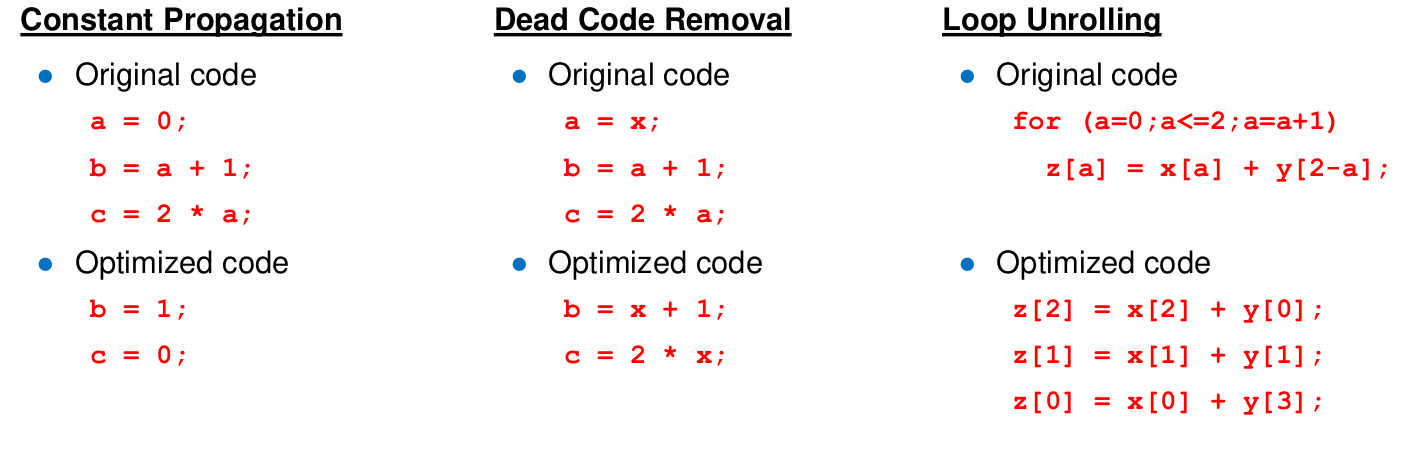
\includegraphics[width=0.95\textwidth]{img/17_elab_ex.png}
\end{figure}
\end{frame}
\note{
\scriptsize{
The elaborator can do some optimization as it constructs the design:
\begin{itemize}
\item It can propagate constants to eliminate unneeded operators.
\item It can remove code that is not executed or that sets variables that are not used.
\item It unrolls loops.
\end{itemize}

}
}

%%%%%%%%%%%%%%%%%%%%%%%%%%%%%%%%%%%%%%%%%%%%%%%%%%%%%%%%%%%%
\begin{frame}[fragile]
\frametitle{Applying Constraints}
\footnotesize{
Inform the tool of the expected operating environment and of any timing paths it can ignore or are longer than one clock cycle in normal operation.
\begin{itemize}
\item Clock signal attributes
\begin{itemize}
\footnotesize{
	\item Period, duty cycle, skew, latency
}
\end{itemize}
\item Arrival times (w.r.t. clock) at I/O ports
\item Environmental attributes
\begin{itemize}
\footnotesize{
	\item Input drive, output load
}
\end{itemize}
\item Timing exceptions
\begin{itemize}
\footnotesize{
	\item False or multi-cycle timing paths
}
\end{itemize}
\end{itemize}
\vspace{6pt}
\textbf{Example}
\begin{Verbatim}[commandchars=\\\{\}, tabsize=2]
\textcolor{blue}{	define_clock -name 100MHz -period 10000}
\end{Verbatim}

}

\end{frame}
\note{
\scriptsize{
Timing and design constraints describe the "design intent" and the surrounding constraints, including synthesis, clocking, timing, environmental, and operating conditions.
\newline

Set these constraints on start points and end points to ensure that every path is properly constrained to obtain an optimal implementation of the RTL design. A path begin point is from either an input port or a register clock pin, while an end point is either an output port or a register data pin.
\newline

Use these constraints to:
\begin{itemize}
\item Describe different attributes of clock signals, such as the duty cycle, clock skew, and the clock latency.
\item Specify input and output delay requirements of all ports relative to a clock transition.
\item Apply environmental attributes, such as load and drive strength to the top-level ports.
\item Set timing exceptions, such as multi-cycle paths and false paths.
\end{itemize}

}
}

%%%%%%%%%%%%%%%%%%%%%%%%%%%%%%%%%%%%%%%%%%%%%%%%%%%%%%%%%%%%
\begin{frame}[fragile]
\frametitle{Mapping to Generic Cells and Optimize}
\footnotesize{
Do technology-independent RTL optimizations:
\begin{itemize}
\item Prune unloaded logic
\item Optimize arithmetic expressions
\item Share common sub-expressions
\item Share and duplicate resources
\item Carry-save adder transformations
\item Merge and map operators to implementations
\end{itemize}
\vspace{6pt}
\textbf{Example}
\begin{Verbatim}[commandchars=\\\{\}, tabsize=2]
\textcolor{blue}{	synthesize -to_generic}
\end{Verbatim}

}
\end{frame}
\note{
\scriptsize{
The synthesis tool does technology-independent RTL optimizations as a preliminary step, including:
\begin{itemize}
\item Datapath synthesis
\item Resource sharing and speculation
\item Multiplexor optimization
\item Carry-save adder (CSA) optimizations
\end{itemize}

}
}

%%%%%%%%%%%%%%%%%%%%%%%%%%%%%%%%%%%%%%%%%%%%%%%%%%%%%%%%%%%%
\begin{frame}
\frametitle{Pruning Unloaded Logic}
\footnotesize{
Technology-independent optimizations remove unloaded logic.
\begin{itemize}
\item Removed cells marked X below do not transitively drive outputs.
\end{itemize}
\begin{figure}
    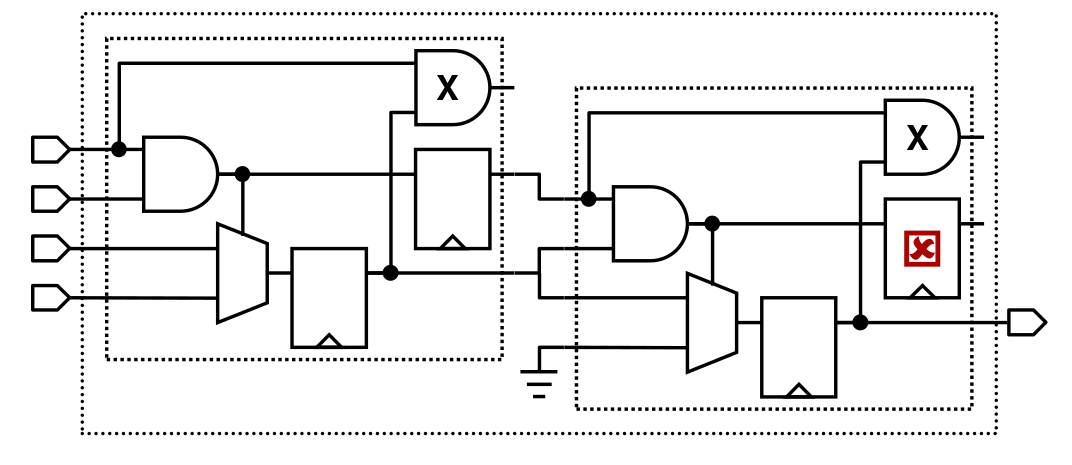
\includegraphics[width=0.85\textwidth]{img/17_prune.png}
\end{figure}
}
\end{frame}
\note{
\scriptsize{
Technology-independent optimizations include the removal of unloaded logic. Here, the cells marked X do not transitively drive outputs so are removed.

}
}

%%%%%%%%%%%%%%%%%%%%%%%%%%%%%%%%%%%%%%%%%%%%%%%%%%%%%%%%%%%%
\begin{frame}
\frametitle{Optimizing Arithmetic Expressions}
\begin{figure}
    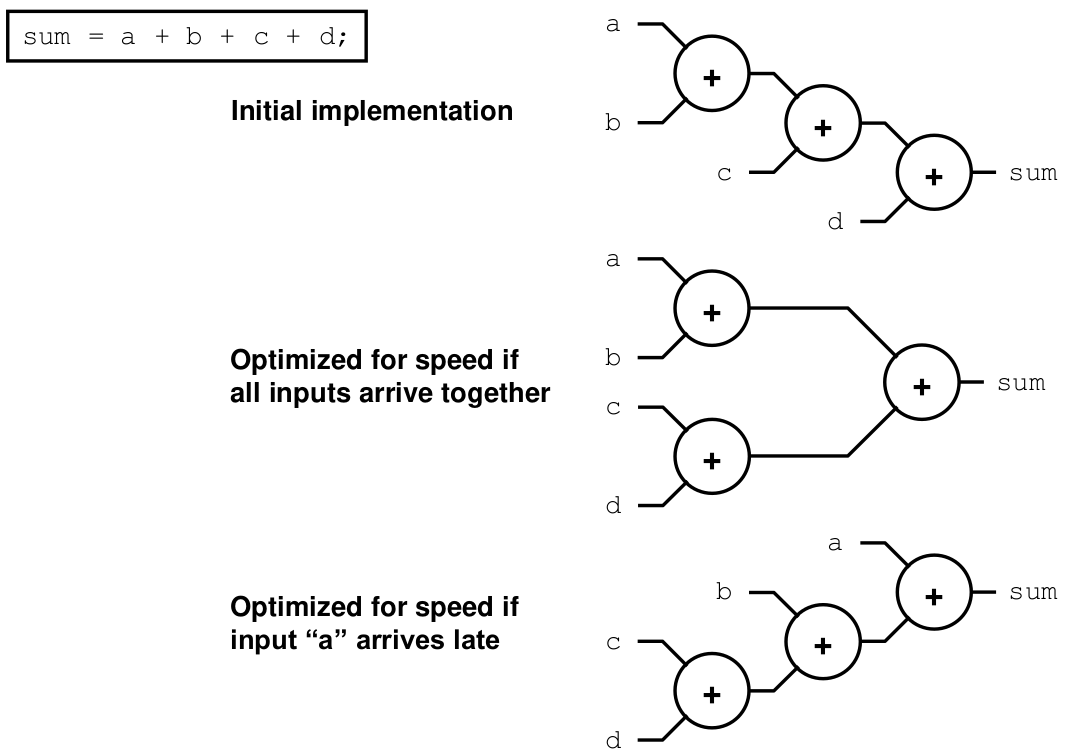
\includegraphics[width=0.85\textwidth]{img/17_optimize.png}
\end{figure}
\end{frame}
\note{
\scriptsize{
Technology-independent optimizations include the restructuring of arithmetic expressions. The logic tree is restructured to as much as practical balance the arrival times from all inputs. During RTL optimizations the tool estimates path delay based upon expression depth.
\newline

Tools typically honour explicit parentheses. Include parentheses to force structure when you know for example that some input will arrive late, and otherwise do not include parentheses.

}
}

%%%%%%%%%%%%%%%%%%%%%%%%%%%%%%%%%%%%%%%%%%%%%%%%%%%%%%%%%%%%
\begin{frame}
\frametitle{Sharing Common Sub-Expressions}
\begin{figure}
    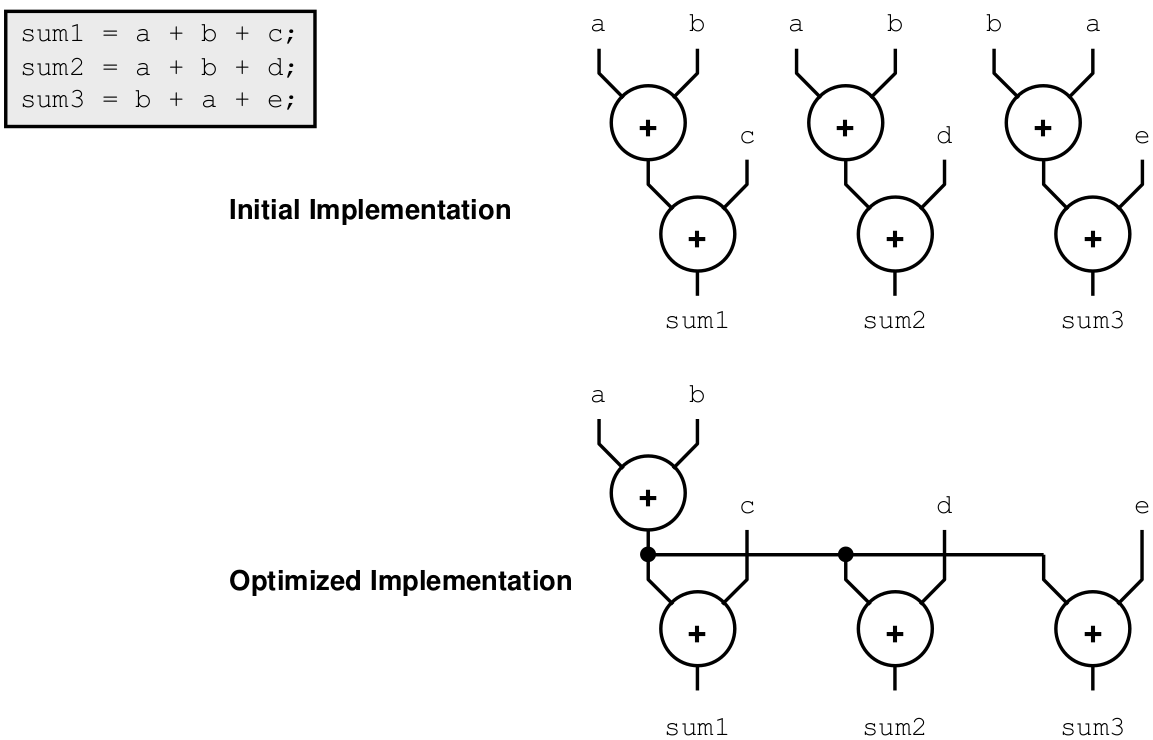
\includegraphics[width=0.85\textwidth]{img/17_sharing.png}
\end{figure}
\end{frame}
\note{
\scriptsize{
Technology-independent optimizations include sub-expression elimination. Here, the (a+b) sub-expression is common to the three sums, so is shared. The tool may later duplicate sub-expressions to meet timing requirements. The order of the sub-expression operands is immaterial, but for most tools the sub-expressions must be in same relative position in its enclosing expression.

}
}

%%%%%%%%%%%%%%%%%%%%%%%%%%%%%%%%%%%%%%%%%%%%%%%%%%%%%%%%%%%%
\begin{frame}
\frametitle{Sharing Resources}
\scriptsize{
\begin{multicols}{2}
A resource is a computational element, such as an adder, shifter, or multiplexor.
\newline

Each HDL operator represents a unique resource type.
\begin{itemize}
\item $+$ operator requires an adder.
\item $>$ operator requires a comparator.
\end{itemize}
\textit{Without} sharing, the number of resources is the number of operators.
\newline

\textit{With} sharing, the number of resources can be reduced.
\begin{itemize}
\item Some operators can share the same resource in alternate clock cycles.
\item Some resources can implement more than one type of operation, e.g., $+$ and $-$.
\end{itemize}

\vfill
\columnbreak
\begin{figure}
    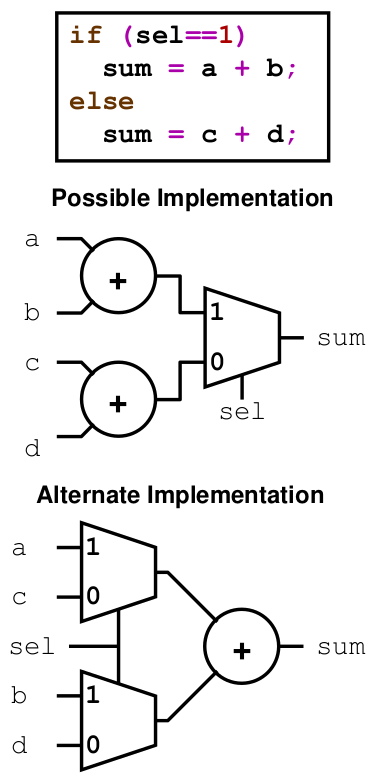
\includegraphics[width=0.35\textwidth]{img/17_sharing_res.png}
\end{figure}
\end{multicols}
}
\end{frame}
\note{
\scriptsize{
A resource is a computational element, such as an adder, shifter, or multiplexor.
\newline

Each HDL operator represents a unique resource type, for example the "plus" ($+$) operator represents an adder and the "greater than" ($>$) operator represents a comparator. Some tools can even merge some adjacent operators and map the merged operators to a more optimized resource.
\newline

Without sharing, the number of required resources is the number of operators.
\newline

With sharing, the number of required resources can be reduced:
\begin{itemize}
\item Similar operators that are utilized in non-overlapping clock cycles can be shared.
\item Add and subtract operators, for example, can be considered to be similar.
\end{itemize}

Depending upon the tool, resource sharing may occur by default or you may need to enable it.


}
}

%%%%%%%%%%%%%%%%%%%%%%%%%%%%%%%%%%%%%%%%%%%%%%%%%%%%%%%%%%%%
\begin{frame}
\frametitle{Un-Sharing Resources (Speculation)}
Can also \textit{add} resources to meet timing requirements.
\begin{figure}
    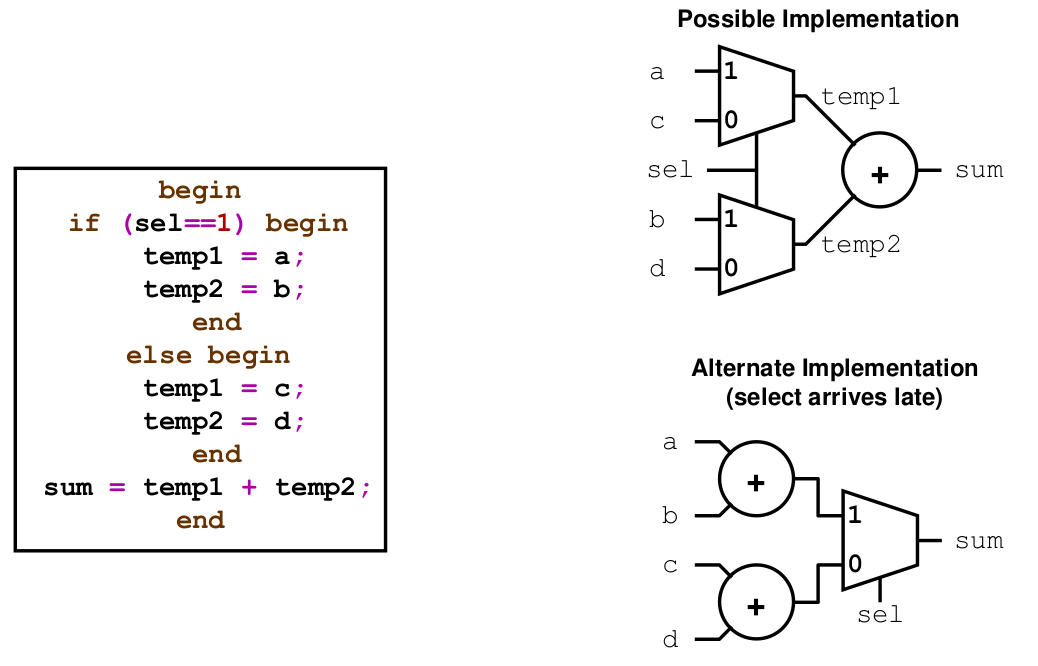
\includegraphics[width=0.75\textwidth]{img/17_unsharing_res.png}
\end{figure}
\end{frame}
\note{
\scriptsize{
The tool can alternatively duplicate resources where needed to meet timing requirements. Here, because the select signal arrives late, synthesis duplicated the adder.

}
}

%%%%%%%%%%%%%%%%%%%%%%%%%%%%%%%%%%%%%%%%%%%%%%%%%%%%%%%%%%%%
\begin{frame}
\frametitle{Carry-Save Adder Transformations}
Carry propagation frequently appears on the critical timing path.
\newline

Carry-save adder transformations "save" carry generation until the end.
\begin{figure}
    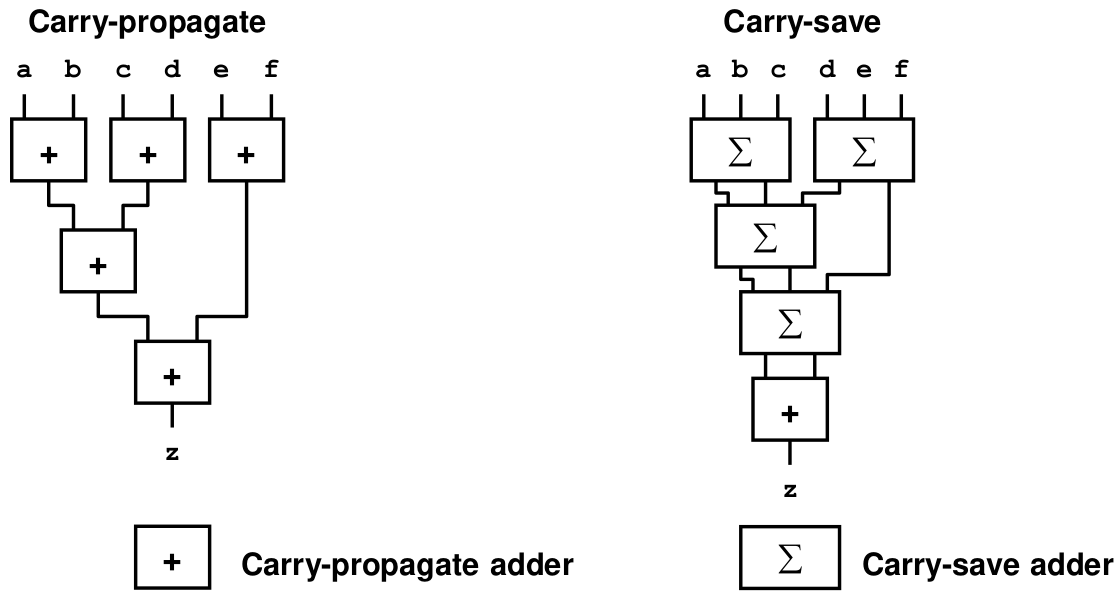
\includegraphics[width=0.85\textwidth]{img/17_carry_save.png}
\end{figure}
\end{frame}
\note{
\tiny{
The most straightforward way to add a set of numbers is to employ an adder tree. Each adder consumes two numbers and produces one. The adder at the root of the tree generates the final sum.


A carry-save adder takes three numbers and produces two outputs, one formed with the sums and the other with the carryouts. Carry-save transformation can greatly improve area and timing.


CSA transformation may apply to any datapath operators whose isolated implementation includes a carry propagate adder. This includes all discrete and relational operators. When the output of one such operator feeds into another datapath operator, it becomes a candidate for CSA transformation. When the output of one mergeable operator feeds into the input of another mergeable operator, it becomes a candidate for CSA transformation.
\newline

Datapath operators are merged in scenarios such as the following:
\begin{itemize}
\item Any combination of Vector Sum, Sum-of-Product, and Product-of-Sum, including intermediary inverted signals.

 $assign\ cs = a + b + c + d;\ assign\ y = cs * p + q;$
\item Comparator

 $assign\ p = a + b;\ assign\ q = c + d;\ assign\ is\_greater = (p > q);$
\item Multiple Fanout

$cs = a * b;\ x = cs + c;\ y = cs + d;$
\item Multiplexers

$assign\ tmp = s\ ?\ a*b\ +\ c*d\ :\ a*c\ +\ b*d;\ assign\ z = tmp + e;$
\item Inverter

$wire\ [16:0]\ tmp = a + b;\ assign\ z = ~tmp + c;$
\item Truncated CSA

$assign\ p = a + b;\ assign\ q = c + d;\ assign\ r = p + q;\ assign\ y = r[17:8];$

\end{itemize}

}
}

%%%%%%%%%%%%%%%%%%%%%%%%%%%%%%%%%%%%%%%%%%%%%%%%%%%%%%%%%%%%
\begin{frame}
\frametitle{Selecting the Architecture: ChipWare}

\end{frame}
\note{
\scriptsize{

}
}

%%%%%%%%%%%%%%%%%%%%%%%%%%%%%%%%%%%%%%%%%%%%%%%%%%%%%%%%%%%%
\begin{frame}
\frametitle{Lab}

\end{frame}
\note{
\scriptsize{

}
}

%%%%%%%%%%%%%%%%%%%%%%%%%%%%%%%%%%%%%%%%%%%%%%%%%%%%%%%%%%%%
\begin{frame}
\frametitle{Lab}

\end{frame}
\note{
\scriptsize{

}
}

%%%%%%%%%%%%%%%%%%%%%%%%%%%%%%%%%%%%%%%%%%%%%%%%%%%%%%%%%%%%
\begin{frame}
\frametitle{Lab}

\end{frame}
\note{
\scriptsize{

}
}

%%%%%%%%%%%%%%%%%%%%%%%%%%%%%%%%%%%%%%%%%%%%%%%%%%%%%%%%%%%%
\begin{frame}
\frametitle{Lab}

\end{frame}
\note{
\scriptsize{

}
}



%%%%%%%%%%%%%%%%%%%%%%%%%%%%%%%%%%%%%%%%%%%%%%%%%%%%%%%%%%%%
\begin{frame}
\frametitle{Test You Understanding - 1}

\begin{itemize}
\item[$\square$] 
\item[$\square$] 
\item[$\square$] 
\item[$\square$] 
\item[$\square$] 
\end{itemize}
\end{frame}
\note{
\scriptsize{

}
}


\end{document}
